% \documentclass[twocolumn]{article}
\documentclass[letter]{article}
\usepackage[a4paper, total={6in, 8in}]{geometry}

%%% Load packages
%\usepackage{amsthm}
%\RequirePackage{natbib}
%\RequirePackage[authoryear]{natbib}% uncomment this for author-year bibliography
\usepackage{hyperref}
\usepackage[utf8]{inputenc} %unicode support
%\usepackage[applemac]{inputenc} %applemac support if unicode package fails
%\usepackage[latin1]{inputenc} %UNIX support if unicode package fails

\usepackage{graphicx}
\usepackage{minted}
\usemintedstyle{vs}

\usepackage{amsmath,amssymb}
\usepackage{booktabs}

\newcommand{\opentsne}{\textsf{openTSNE}}

\renewcommand{\baselinestretch}{1.2}

\begin{document}

\title{openTSNE: a modular Python library for t-SNE dimensionality reduction and embedding}

\author{
  Pavlin G. Poli\v{c}ar\textsuperscript{1}\\
  \texttt{pavlin.policar@fri.uni-lj.si}\\
  \and
  Martin Stra\v{zar}\textsuperscript{2}\\
  \texttt{martin.strazar@gmail.com}\\
  \and
  Bla\v{z} Zupan\textsuperscript{1,3}\\
  \texttt{blaz.zupan@fri.uni-lj.si}\\
}

\date{
  \textsuperscript{1}Faculty of Computer and Information Science, University of Ljubljana,\\
  Ve\v{c}na pot 113, SI-1000 Ljubljana, Slovenia\\ \vspace{2mm}
  \textsuperscript{2}Broad Institute of Harvard and MIT,\\
  D\"{u}sternbrooker Weg 20, MA-02142 Cambridge, U.S.A.\\ \vspace{2mm}
  \textsuperscript{3}Department of Molecular and Human Genetics, Baylor College of Medicine,\\
  1 Baylor Plaza, TX-77030 Houston, U.S.A.
}

\maketitle

\begin{abstract}
Point-based visualizations of large, multi-dimensional data from molecular
biology are often used to reveal meaningful clusters. One of the most popular
techniques to construct such visualizations is $t$-distributed stochastic
neighbor embedding (t-SNE). Several extensions of t\nobreakdash-SNE have
recently been proposed to address issues of scalability and the quality
of the resulting visualizations. We introduce \opentsne, a modular
Python library that implements the core t\nobreakdash-SNE algorithm and its many
extensions.
The library is fast and enables users to embed data sets containing millions of
data points in a matter of minutes on consumer-grade laptop computers.
Unique to \opentsne\ is also the ability to map new data to existing embeddings,
which can surprisingly assist in solving batch effects.
\end{abstract}

\providecommand{\keywords}[1]{\vspace{2mm}\textbf{Keywords ---} #1}
\begin{keywords}
t-SNE, embedding, visualization, dimensionality reduction, Python library
\end{keywords}


\section*{Introduction}

The abundance of high-dimensional data sets in molecular biology calls for
dimensionality reduction techniques that are able to produce
informative data visualizations. Popular approaches include principal component
analysis (PCA), multidimensional scaling, t-distributed stochastic neighbor
embedding (t-SNE)~\cite{maaten2008visualizing}, and uniform manifold
approximation and projections (UMAP)~\cite{2018arXivUMAP}. Among these, t-SNE has
received much attention as it can address high volumes of data and reveal
meaningful clustering structure. The increased resolution and throughput of modern
molecular assays has lead to the frequent use of t-SNE in diverse fields
including, but not limited to, single-cell
transcriptomics (scRNA-seq,~\cite{macosko2015highly,cao2019single,tasic2018shared}),
human genetics~\cite{hirata2019genetic}, metagenomic
assembly~\cite{beaulaurier2018metagenomic}, the spatial organization of
microbial communities~\cite{sheth2019spatial} and
metabolomics~\cite{tkachev2019differences}. Reports on single-cell gene
expression data, our running example, often start with an overview of the cell
landscape, where t-SNE is used to embed high-dimensional expression profiles into a
two-dimensional space. Figs.~\ref{fig:macosko}.a and \ref{fig:macosko}.b show
two such embeddings.

\begin{figure*}[htbp]
  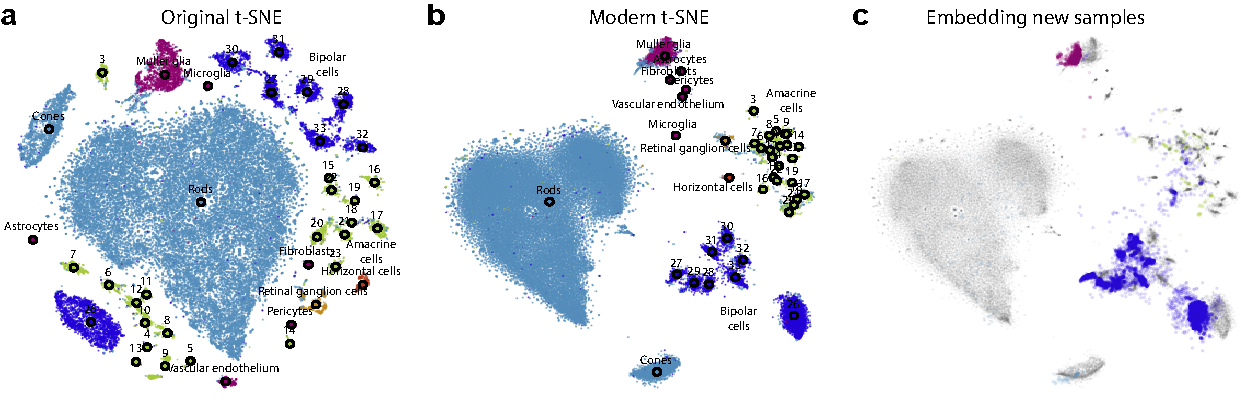
\includegraphics[width=\textwidth]{macosko2015}
  \caption{\label{fig:macosko}
  We use \opentsne\ to generate three t-SNE embeddings and demonstrate recent
  theoretical advances. The data in \textbf{(a)} and \textbf{(b)} represent 44,808
  single-cell gene-expression profiles of mouse retinal cells from Macosko
  \textit{et al.}~\cite{macosko2015highly}. The data in \textbf{(c)}
  additionally contains 27,499 expression profiles from mouse
  retinal cells from Shekhar \textit{et al.}~\cite{shekhar2016comprehensive}.
  \textbf{(a)} We construct a t-SNE
  embedding following the parameter choices from the original publication
  by Maaten \& Hinton~\cite{maaten2008visualizing}. The visualization
  shows no preservation of the global organization of clusters,
  resulting from random initialization and an affinity model focused on
  preserving local neighborhoods. \textbf{(b)} A modern t-SNE
  embedding, utilizing the latest theoretical advances and practical
  recommendations constructed using a multi-scale
  affinity model, preserving both short-range and long-range interactions
  between data points and initialized so that the global layout is
  as meaningful as possible. Unlike in \textbf{(a)}, the green and blue clusters
  representing different sub-types of amacrine and bipolar cells are now
  localized to the same regions of the space, indicating a higher level
  of similarity than to other cell types. The embedding in \textbf{(c)} shows how existing
  t-SNE reference atlases can be used to place new samples into existing
  embeddings. The positions of new data points correspond to cell types
  from the reference atlas.
}
\end{figure*}

Despite its utility, t-SNE has often been criticized for its limited
scalability, lack of global organization -- t-SNE identifies well-defined clusters that
may be arbitrarily scattered throughout the low-dimensional space -- and the absence of
theoretically-founded methods to map new data into existing
embeddings~\cite{ding2018interpretable,becht2019dimensionality}. Most of these
shortcomings have recently been addressed. Linderman \textit{et al.} developed
an interpolation-based approximation scheme which massively improved the
scalability of t-SNE, achieving linear time complexity
in the number of samples~\cite{linderman2019fast}. Kobak \& Berens proposed
several techniques to improve global cluster coherence, including estimating
similarities with a mixture of Gaussian kernels~\cite{kobak2019art}. In our
previous work, we presented a principled approach for embedding new samples into
existing visualizations~\cite{policar2019embedding}.


\section*{Results}

We introduce \opentsne, a comprehensive Python library that implements t-SNE
and all its recently proposed extensions, including:
\begin{enumerate}
\item the implementation of efficient approximation 
	schemes~\cite{van2014accelerating,linderman2019fast} allowing the embedding
	of millions of data points,
\item the addition of new data samples into a fixed existing
	embeddings~\cite{policar2019embedding},
\item improved initialization schemes~\cite{kobak2019umap} leading to more
	globally consistent layouts,
\item variable degrees of freedom~\cite{kobak2019heavy} allowing the inspection
	of data at different levels of resolution,
\item multi-scale similarity kernels~\cite{kobak2019art} which preserve small,
	well-defined clusters and uncover global relationships between clusters,
	and
\item improved defaults for learning rate and number of
	iterations~\cite{belkina2019automated} which produce embeddings at a lower
	computational cost.
\end{enumerate}

\opentsne\ is compatible with the Python data science ecosystem and
libraries including \textsf{numpy}, \textsf{scikit-learn}, \textsf{scanpy}),
providing a familiar and intuitive application program interface to new
users. Its modular design encourages extensibility and experimentation with
various settings and changes to the analysis pipeline. We have released
\opentsne\ to the open-source community to make recent theoretical advancements
more accessible to a wider audience. At
the time of the writing, the library averages thousands of weekly
downloads and has received over 750 GitHub stars, an appreciation score gained
by only $0.3\%$ of public Python repositories. The source code is available at
\url{https://github.com/pavlin-policar/openTSNE} and supports installations from
\textsf{PyPI} and \textsf{conda-forge}, the two most widely adopted Python
package managers.

Accessibility of the latest theoretical advancements in t-SNE is one of the core
design principles of \opentsne. This range of advancements is easily accessible through an intuitive
programming interface, where we closely follow the style
\textsf{scikit-learn}~\cite{sklearn_api}, a popular and widely used
library for machine learning. The following snippet exemplifies this interface
and was used to generate the four visualizations in Fig.~\ref{fig:tasic}, demonstrating the
effect of a particular recent theoretical advancements in the t-SNE algorithm. 

\begin{minted}[
fontsize=\footnotesize,
frame=lines,
framesep=2mm,
baselinestretch=1.1
]{python}
import openTSNE
from openTSNE.affinity import Multiscale
# a - standard t-SNE
tsne1 = openTSNE.TSNE(perplexity=30).fit(X)
# b - high perplexity for global structure
tsne2 = openTSNE.TSNE(perplexity=500).fit(X)
# c - multiscale kernel for local/global structure
aff = Multiscale(X, perplexities=[30, 500])
tsne3 = openTSNE.TSNE(affinities=aff).fit(X)
# d - decrease dof for higher resolution
tsne4 = openTSNE.TSNE(dof=0.6).fit(X)
\end{minted}

\noindent The code snippet considers a \textsf{numpy} array or \textsf{scipy}
sparse matrix \texttt{X} and creates four \texttt{TSNEEmbedding} objects. These
objects represent t-SNE embeddings that may subsequently be optimized under
different parameter settings or used to embed new samples into the embedding
landscape. Function calls may include additional parameters not shown in the
example code but are explained in the accompanying notebooks available at
\url{https://github.com/pavlin-policar/opentsne-paper}.

\section*{Discussion}

\subsection*{Uncovering Structure in High-Dimensional Data}

Dimensionality reduction techniques implicitly assume that high-dimensional data
lies on a lower-dimensional manifold, which can accurately be captured by a
small number of dimensions. However, there is no evidence that every data set
can accurately be described using only two dimensions, and any such embedding
will inevitably lead to a loss of information. Thus, it is beneficial to examine
multiple embeddings, each of which provides a different perspective on topology
and other data characteristics.

\begin{figure*}[htbp]
  \center
  \includegraphics[width=0.75\textwidth]{tasic2018}
	\caption{\label{fig:tasic}
  We use \opentsne\ to create four different
	visualizations of the Tasic \textit{et al.}~\cite{tasic2018shared} data,
	each providing a different perspective into the topology of the data.
	The data set contains 21,874 single-cells originating from the mouse
	neocortex. Cluster annotations and colors are taken from the original
	publication. Warm colors correspond to excitatory neurons, cool colors
	correspond to inhibitory neurons, and gray/brown colors correspond to
	non-neuronal cells. Standard t-SNE \textbf{(a)} emphasizes local
	structure while increasing perplexity \textbf{(b)} results in a more
	meaningful layout of the clusters. We can also combine the two
	perplexities by using a multiscale kernel affinity model \textbf{(c)}
	and obtain a trade-off between global and local structure.
	Alternatively, we can inspect more fine-grained structure and reveal
  smaller clusters by using a more heavy-tailed kernel \textbf{(d)}.}
\end{figure*}

We illustrate this point by generating four different embeddings of the data on
single-cell gene expression in mouse brain~\cite{tasic2018shared}.
Fig.~\ref{fig:tasic}.a shows an embedding using default t-SNE parameters. While
different clusters of excitatory and inhibitory neurons appear close to one
another, all clusters appear equidistant from their neighbors, and the overall
relations between groups are not obvious. The embedding in Fig.~\ref{fig:tasic}.b
focuses on preserving larger neighborhoods of points, resulting in a more
globally consistent layout where relations between clusters become more
apparent. Here, it is evident from the increased white space between groups that
there is one large class of excitatory neurons and two related classes of
inhibitory neurons. Unfortunately, focusing on preserving large neighborhoods
leads to the absorption of smaller clusters into larger ones. Alternatively,
Fig.~\ref{fig:tasic}.c uses multi-scale similarity kernels that aim to preserve
both the global organization of clusters and prevent smaller cluster absorption. We
constructed the embedding from Fig.~\ref{fig:tasic}.d with the settings used
for Fig.~\ref{fig:tasic}.a, but at a finer level of resolution.
The figure demonstrates that some clusters are composed of numerous, smaller
subgroups representing different cell subpopulations which are not visible under
standard parameter settings.

When dealing with data containing millions of data points, standard t-SNE
embeddings often become unwieldy -- cluster boundaries are blurred, large
clusters absorb smaller ones, and relationships between clusters become
increasingly difficult to interpret. We constructed Fig.~\ref{fig:cao}.a from
the data containing expression profiles of over two million single cells
captured at different time points in mouse development. The embedding indicates
numerous clusters with transitions between time points, as marked by the
color-coding, that are difficult to interpret. Kobak \& Berens observed that
increasing attractive forces between similar data points controlled via the
\textit{exaggeration} parameter leads to more compact clusters, and
subsequently, more informative visualizations~\cite{kobak2019art}. For instance,
\ref{fig:cao}.b doubles the default exaggeration, which uncovers some of the
data's overall structure. Further doubling the exaggeration in \ref{fig:cao}.c
allows us to observe that the data is comprised of two main groups of cells and
eight somewhat smaller clusters. The visualization also reveals several tiny
clusters, possibly corresponding to rare cell types.

\begin{figure*}[htbp]
  \includegraphics[width=\textwidth]{cao2019}
  \caption{\label{fig:cao}
  Increasing the exaggeration parameter leads to compact clusters, highlighting
	the data's global organization and emphasizing the continuous nature of
	cell state transitions. The data set from Cao \textit{et al.}~\cite{cao2019single}
	contains expression profiles from 2,058,652 single cells. The data were
	collected from mice embryos at different developmental stages at daily
	intervals after 9.5 to 13.5 days. \textbf{(c)} reveals that the data is
	comprised of two main components -- the neural tube and mesenchymal
	cells -- as well as several other smaller clusters. The
	colors indicate developmental progression with red indicating
	least-developed cells and blue indicating most developed cells. The
	overall developmental trajectory is most apparent with higher
	exaggeration levels, showing red cells slowly transitioning into blue
	cells. Progressively easing the exaggeration factor uncovers finer
	clusters within the larger groups, as shown in \textbf{(b)} with
	exaggeration of two and subsequently in \textbf{(a)}, where we show the
	standard t-SNE with no exaggeration. 32,011 putative doublets are
	excluded from the visualizations.
}
\end{figure*}

Exaggeration can highlight transitions between cell states in developmental
studies. Standard t-SNE often produces embeddings with clearly defined, discrete
clusters. We can adjust the level of granularity and resolution of the clusters
with several parameters in Fig.~\ref{fig:tasic}. However, discrete clusters are
often undesired in developmental studies where cells' state is assumed to follow
a continuous transition path. To this end, other embedding techniques such as UMAP and
ForceAtlas2~\cite{jacomy2014forceatlas2} are used to better capture the continuity
between cell states. Recently, B{\"o}hm \textit{et al.}~\cite{bohm2020unifying}
showed that embeddings produced by t-SNE with exaggeration values of 4 and
$\sim30$ construct embeddings which are markedly similar to UMAP and
ForceAtlas2, respectively. For example, in Fig.~\ref{fig:cao}.a, the
developmental trajectory between different time points is difficult to observe
due to many sprawled out clusters. On the other hand, it is easier to trace the
development when we increase the exaggeration factor from $1$ to $2$ to $4$ in
Figs.~\ref{fig:cao}.b-c.

\subsection*{Embedding New Samples}

Unlike other popular dimensionality reduction techniques such as principal
component analysis or autoencoders, t-SNE is a non-parametric method and does
not define an explicit mapping to the embedding space. Therefore, embeddings of
new data points need to be found through
optimization~\cite{policar2019embedding}. \opentsne\ is currently the only
publicly available library allowing users to add new samples to existing
embeddings in a principled manner.

Figs.~\ref{fig:macosko}.b and \ref{fig:macosko}.c demonstrate how we can use a
previously labeled single-cell data set and embed cells from a separate
experiment into the reference landscape. The reference data from
Macosko~\textit{et al.}~\cite{macosko2015highly} contains gene expression
profiles from mouse retinal cells. By embedding the samples from a similar
experiment on bipolar retinal cells by Shekhar~\textit{et
al.}~\cite{shekhar2016comprehensive}, we can correctly map the bipolar cell
clusters onto the reference embedding.

Embedding single cells into existing reference atlases can also be useful for
cell-type classification in cases of unknown cell identities. For instance, in
Fig.~\ref{fig:transform}, we construct a reference embedding using labeled data
from Hochgerner~\textit{et al.}~\cite{hochgerner2018conserved} containing
gene-expression profiles of cells from the mouse brain. The authors assign a
type to each cell. We can verify their classification accuracy by visualizing
the expression of well-established gene markers for the major cell types. We
then embed cells from Harris~\textit{et al.}~\cite{harris2018classes} into the
constructed cell atlas. In Harris~\textit{et al.}~, labels are provided only for
neuronal cells. In the resulting mapping, we can quickly identify other
non-neuronal cell types, including oligodendrocytes and astrocytes. We can
further use marker genes to validate that the mapping in the reference landscape
is correct. 

\begin{figure*}[htbp]
  \includegraphics[width=\textwidth]{transform_hochgerner}
  \caption{\label{fig:transform}
  \opentsne\ supports embedding new samples into an existing reference t-SNE
	landscape. For the series of visualizations shown in this figure, we
	first construct a t-SNE embedding for the data from Hochgerner
	\textit{et al.}~\cite{hochgerner2018conserved} containing 24,185
	developing, single cells from the mouse hippocampus. The data contains
	gene expression in different neurons, supporting glia, and other
	vascular cells (upper left). Data points representing cells are colored
	according to cell-types assigned in the original publication; see the
	legend from Fig.~\ref{fig:tasic} to map colors to cell-type. We then
	embed new, hippocampal cells collected in a study by Harris \textit{et
	al.}~\cite{harris2018classes} using the embedding of Hochgerner
	\textit{et al.} data as a reference. In their study, Harris \textit{et
	al.} collected 6,971 single-cells and focused on identifying different
	types of inhibitory neurons. However, almost half of the collected cells
	are not neurons and were left uncharacterized. Inspecting the embeddings
	of these cells in the reference embedding (bottom left) reveals that in
	addition to inhibitory neurons, the data contains several supporting
	glial cells as well as a small population of endothelial cells. We can
	verify our approach's accuracy by inspecting marker genes for the major
	cell types in the reference (top row) and embedded samples (bottom row).
}
\end{figure*}

The examples presented above demonstrate how to use \opentsne\ to quickly gain
insight into newly-sequenced, single-cell data sets by utilizing existing cell
atlases. The approach is general and not limited to single-cell gene expression,
and one can, in principle, apply it to any tabular data set regardless of field.

\subsection*{Versatility}

Versatility, the ability to use and combine different optimization approaches to
construct different embedding spaces, is another of \opentsne's core design
principles. Kobak \& Berens recently provided several recommendations and
tricks to obtain better and more meaningful t-SNE
visualizations~\cite{kobak2019art}. These include multi-scale similarity
kernels, perplexity annealing, and increasing exaggeration when working with
massive data sets. \opentsne\ provides a flexible program interface to
incorporate these improvements in just a few lines of code. Furthermore, \opentsne\
supports custom affinity models, enabling users to construct t-SNE embeddings on
non-tabular relational data: the only requirement imposed by the affinity-model
is some notion of similarity between data points.
Finally, \opentsne's comprehensive callback system can be utilized
to monitor and adapt different stages of the optimization phase and has been
used to construct visually appealing animations of the t-SNE optimization
process.


\subsection*{Speed}

One of the t-SNE's common criticisms is limited scalability to large data sets
containing, for instance, millions of data
points~\cite{becht2019dimensionality}. The culprit for slow response time stems
from a particular optimization procedure and its specific implementation in
popular Python libraries. Until quite recently, most popular
implementations of t-SNE were based on the Barnes-Hut approximation scheme
developed by van der Maaten in 2014~\cite{van2014accelerating} with asymptotic
time complexity $\mathcal{O}(N \log N)$, where $N$ is the number of data items ({\em
e.g.} cells). The most widely-used implementation of t-SNE came from
\textsf{scikit-learn}, which exhibits long runtimes when compared to its C++
counterpart -- \textsf{MulticoreTSNE}. The multi-threaded \textsf{MulticoreTSNE}
implementation~\cite{Ulyanov2016} can construct t-SNE embeddings of millions of
data points in a matter of hours on widely-accessible, consumer-grade processors
(Fig.~\ref{fig:benchmarks}). However, recently, Linderman \textit{et al.}
developed a new approximation scheme -- FIt-SNE -- which further reduces the
asymptotic time complexity to $\mathcal{O}(N)$. We include this approach in
\opentsne\, enabling the embedding of large data sets in a matter of minutes. 

Fig.~\ref{fig:benchmarks} benchmarks four popular Python t-SNE implementations,
including those from \textsf{scikit-learn} (v0.23.1), \textsf{MulticoreTSNE}
(v0.1), \textsf{FIt-SNE} (v1.1.0), and our \opentsne\ (v0.4.3). We perform
benchmarks on two computational platforms, one representing the usage on a
personal computer and the other the utility of these libraries on a high-performance
computing platform. The Intel(R) Core i7 is commonly found in consumer-grade
laptop computers, while Intel(R) Xeon(R) processors appear in high-performance
computing machines. Benchmarks were run for $1,000$ iterations with the original
t-SNE parameters, as some implementations do not allow their modification. 

\begin{figure*}[htbp]
  \includegraphics[width=\textwidth]{benchmarks}
  \caption{\label{fig:benchmarks}
  We benchmark \opentsne\ (v0.4.3) against three popular open-source implementations
	from \textsf{scikit-learn}~\cite{pedregosa2011scikit} (v0.23.1),
	\textsf{MulticoreTSNE}~\cite{Ulyanov2016} (v0.1), and
	\textsf{FIt-SNE}~\cite{linderman2019fast} (v1.1.0). Experiments were run on a
	consumer-grade Intel Core i7-7700HQ processor found in laptop computers,
	and on a server-grade Intel Xeon E5-2650. To generate benchmark data
	sets of different sizes, we subsampled data from the 10X Genomics 1.3
	million mouse brain data set five times, resulting in five different
	data sets for each size. In total, we run each implementation on 30
	different data sets. Notice that \opentsne\ scales similarly to \textsf{FIt-SNE},
	as they both use the same interpolation-based approximation scheme,
	while \textsf{scikit-learn} and \textsf{MulticoreTSNE} utilize the Barnes-Hut
	approximation.
}
\end{figure*}

Benchmark results (Fig.~\ref{fig:benchmarks}) confirm that both \textsf{FIt-SNE}
and \opentsne\ scale better than their Barnes-Hut counterparts --
\textsf{scikit-learn} and \textsf{MulticoreTSNE}. While \opentsne's
implementation uses Python that incurs some runtime overhead compared to its C++
counterpart \textsf{FIt-SNE}, the two libraries' speeds are surprisingly
comparable. Modern computer processors contain multiple cores, allowing us to
use multi-threading, which further reduces the gap between \opentsne\ and
\textsf{FIt-SNE}. On the server-grade processor, \opentsne\ is slightly faster
than its pure C++ counterpart when utilizing multiple cores. \opentsne\ uses
\textsf{numpy} for most linear algebra operations, which may make better use of
the Intel Math Kernel Library (MKL), which is aggressively optimized on Intel(R)
Xeon(R) processors.  

\opentsne\ provides a flexible API, allowing splitting up the
embedding-construction process into several parts, caching slow operations.
Running t-SNE optimization in stages enables users to quickly experiment with
different parameter settings and iterate on their final visualizations.

\subsection*{Ease of Use}

Intuitive access and simple installation procedures almost universally correlate
with the widespread adoption of novel computational techniques. While the t-SNE implementation
from \textsf{scikit-learn} fits this requirement, the implementation proves
prohibitively slow for even moderately-sized data sets that span tens of
thousands of data records. Other C++ implementations such as
\textsf{MulticoreTSNE} and \textsf{FIt-SNE} exhibit better scaling in more
massive data sets, but do not provide precompiled binaries and require users to
compile the software themselves. This problem is critical, for instance, for
users of the Windows operating system, where the C++ compiler does not come with the system, making
the correct configuration of current t-SNE implementations cumbersome.

We designed \opentsne\ to be accessible to a broader audience. We
provide precompiled binaries for all major Python versions on all major
platforms, making the installation process as seamless as possible. One can
install \opentsne\ through the Python Package Index (\textsf{PyPI}) or \textsf{conda} from the
\textsf{conda-forge} channel, the two most widely adopted Python package managers.
\opentsne's interface is inspired by \textsf{scikit-learn},
which is well established in the Python data science ecosystem. \opentsne\
implements multi-threaded versions of both the Barnes-Hut and FIt-SNE
approximation schemes, enabling it to be applied to data sets containing millions of data
points. While the Python virtual machine inevitably introduces some performance overhead,
the runtime is comparable to its C++ counterpart -- \textsf{FIt-SNE}. Finally,
\opentsne\ is extensible. Its modular design enables researchers to quickly
experiment with different parameter settings and easily incorporate custom components into
the software. We provide a full feature list and comparison to other popular
t-SNE implementations in Table~\ref{tab:features}.

\begin{table}
\caption{\label{tab:features}
  Features of \opentsne\ compared to other three popular open-source implementations
	from \textsf{scikit-learn}~(v0.23.1), \textsf{MulticoreTSNE} (v0.1), and
	\textsf{FIt-SNE} (v1.1.0).  The first section of the comparison
	addresses packaging and distribution. A properly packaged library is
	easily accessible to users, and developers should easily include it in
	dependency lists of other software packages. The second section of the
	comparison lists the two existing t-SNE approximation schemes. The
	FIt-SNE approximation scheme is required for t-SNE to scale up to
	millions of data points. The final section provides a list of extensions
	and improvements to the standard t-SNE algorithm, many of which can
	produce markedly better visualizations.
}
\begin{center}\small
\newcommand*\rot{\rotatebox{90}}
\renewcommand{\arraystretch}{1.25}

\begin{tabular}{r c c c c c c}
\toprule
\setlength\tabcolsep{6pt}
& \rot{\textsf{scikit-learn}} & \rot{\textsf{MulticoreTSNE}} & \rot{\textsf{FIt-SNE}} & \rot{\textsf{openTSNE}} \\
\toprule
\textsf{PyPI} package & \checkmark & \checkmark & & \checkmark \\
\textsf{conda} package & \checkmark & & & \checkmark \\
Precompiled binaries & \checkmark & & & \checkmark \\
\hline
Barnes-Hut ($\mathcal{O}(N \log N)$) & \checkmark & \checkmark & & \checkmark \\
FIt-SNE ($\mathcal{O}(N)$) & & & \checkmark & \checkmark \\
\hline
Multiscale Gaussian kernels & & & \checkmark & \checkmark \\
Fully-custom affinity kernels & & & & \checkmark \\
Variable degrees of freedom & & & \checkmark & \checkmark \\
Variable exaggeration & & & \checkmark & \checkmark \\
Better initialization & & & \checkmark & \checkmark \\
Automatic learning rate & & & \checkmark & \checkmark \\
Embedding new samples & & & & \checkmark \\
\bottomrule
\end{tabular}
\end{center}
\end{table}

\section*{Conclusion}

Data visualization for efficient exploration and effective communication is integral to scientific progress~\cite{wong2012points}. It is of no surprise, then, that a technique called t-SNE that can embed multi-dimensional data within two-dimensional maps has gained such popularity. The t-SNE visualizations appear in numerous recent publications, including those in this journal, and are, in particular, instrumental for the advancement in specific fields of biology, such as single-cell transcriptomics. Yet, with growing data volume and the need for data integration from various experiments, the original t-SNE exhibits lack of scalability and susceptibility to batch effects. We here introduce \opentsne\, an open-source Python t-SNE library that addresses these concerns and includes recent methodological advancements. \opentsne\ can scale to millions of data records and fit local cluster exploration and global structure discovery. It is also the only existing t-SNE library that enables transfer learning in a principled manner, where new data can be embedded into existing atlases.

\section*{Availability}

\opentsne\ is distributed under the BSD-3-Clause License and is publicly
available as an open-source package at
\url{https://github.com/pavlin-policar/openTSNE}. \opentsne\ is also available
on \textsf{PyPI} and \textsf{conda-forge}. The data sets used and scripts used
in this study are included in accompanying notebooks, publicly available at
\url{https://github.com/pavlin-policar/opentsne-paper}.

\section*{Competing interests}
The authors declare no competing interests.

\section*{Author's contributions}
P.G.P. implemented and maintains \opentsne\ library. M.S. helped in the development of mathematical foundations and advised on the inclusion of the extensions. B.Z. initiated and supervised the project. All three co-authors wrote the manuscript.

\section*{Acknowledgements}
This work was supported by Slovenian Research Agency (P2-0209).
We want to thank Dmitry Kobak for various helpful discussions and best practices
when using t-SNE and his contributions to the source code. We would also
like to thank George Linderman for his help with the FIt-SNE algorithm.


%% Bibliography
\begin{thebibliography}{28}
% BibTex style file: bmc-mathphys.bst (version 2.1), 2014-07-24
\ifx \bisbn   \undefined \def \bisbn  #1{ISBN #1}\fi
\ifx \binits  \undefined \def \binits#1{#1}\fi
\ifx \bauthor  \undefined \def \bauthor#1{#1}\fi
\ifx \batitle  \undefined \def \batitle#1{#1}\fi
\ifx \bjtitle  \undefined \def \bjtitle#1{#1}\fi
\ifx \bvolume  \undefined \def \bvolume#1{\textbf{#1}}\fi
\ifx \byear  \undefined \def \byear#1{#1}\fi
\ifx \bissue  \undefined \def \bissue#1{#1}\fi
\ifx \bfpage  \undefined \def \bfpage#1{#1}\fi
\ifx \blpage  \undefined \def \blpage #1{#1}\fi
\ifx \burl  \undefined \def \burl#1{\textsf{#1}}\fi
\ifx \doiurl  \undefined \def \doiurl#1{\textsf{#1}}\fi
\ifx \betal  \undefined \def \betal{\textit{et al.}}\fi
\ifx \binstitute  \undefined \def \binstitute#1{#1}\fi
\ifx \binstitutionaled  \undefined \def \binstitutionaled#1{#1}\fi
\ifx \bctitle  \undefined \def \bctitle#1{#1}\fi
\ifx \beditor  \undefined \def \beditor#1{#1}\fi
\ifx \bpublisher  \undefined \def \bpublisher#1{#1}\fi
\ifx \bbtitle  \undefined \def \bbtitle#1{#1}\fi
\ifx \bedition  \undefined \def \bedition#1{#1}\fi
\ifx \bseriesno  \undefined \def \bseriesno#1{#1}\fi
\ifx \blocation  \undefined \def \blocation#1{#1}\fi
\ifx \bsertitle  \undefined \def \bsertitle#1{#1}\fi
\ifx \bsnm \undefined \def \bsnm#1{#1}\fi
\ifx \bsuffix \undefined \def \bsuffix#1{#1}\fi
\ifx \bparticle \undefined \def \bparticle#1{#1}\fi
\ifx \barticle \undefined \def \barticle#1{#1}\fi
\ifx \bconfdate \undefined \def \bconfdate #1{#1}\fi
\ifx \botherref \undefined \def \botherref #1{#1}\fi
\ifx \url \undefined \def \url#1{\textsf{#1}}\fi
\ifx \bchapter \undefined \def \bchapter#1{#1}\fi
\ifx \bbook \undefined \def \bbook#1{#1}\fi
\ifx \bcomment \undefined \def \bcomment#1{#1}\fi
\ifx \oauthor \undefined \def \oauthor#1{#1}\fi
\ifx \citeauthoryear \undefined \def \citeauthoryear#1{#1}\fi
\ifx \endbibitem  \undefined \def \endbibitem {}\fi
\ifx \bconflocation  \undefined \def \bconflocation#1{#1}\fi
\ifx \arxivurl  \undefined \def \arxivurl#1{\textsf{#1}}\fi
\csname PreBibitemsHook\endcsname

%%% 1
\bibitem{maaten2008visualizing}
\begin{barticle}
\bauthor{\bsnm{Van Der~Maaten}, \binits{L.}},
\bauthor{\bsnm{Hinton}, \binits{G.}}:
\batitle{{Visualizing data using t-SNE}}.
\bjtitle{Journal of Machine Learning Research}
\bvolume{9}(\bissue{Nov}),
\bfpage{2579}--\blpage{2605}
(\byear{2008})
\end{barticle}
\endbibitem

%%% 2
\bibitem{2018arXivUMAP}
\begin{botherref}
\oauthor{\bsnm{{McInnes}}, \binits{L.}},
\oauthor{\bsnm{{Healy}}, \binits{J.}},
\oauthor{\bsnm{{Melville}}, \binits{J.}}:
{UMAP: Uniform Manifold Approximation and Projection for Dimension Reduction}.
ArXiv e-prints
(2018).
\arxivurl{1802.03426}
\end{botherref}
\endbibitem

%%% 3
\bibitem{macosko2015highly}
\begin{barticle}
\bauthor{\bsnm{Macosko}, \binits{E.Z.}},
\bauthor{\bsnm{Basu}, \binits{A.}},
\bauthor{\bsnm{Satija}, \binits{R.}},
\bauthor{\bsnm{Nemesh}, \binits{J.}},
\bauthor{\bsnm{Shekhar}, \binits{K.}},
\bauthor{\bsnm{Goldman}, \binits{M.}},
\bauthor{\bsnm{Tirosh}, \binits{I.}},
\bauthor{\bsnm{Bialas}, \binits{A.R.}},
\bauthor{\bsnm{Kamitaki}, \binits{N.}},
\bauthor{\bsnm{Martersteck}, \binits{E.M.}}, \betal:
\batitle{Highly parallel genome-wide expression profiling of individual cells
  using nanoliter droplets}.
\bjtitle{Cell}
\bvolume{161}(\bissue{5}),
\bfpage{1202}--\blpage{1214}
(\byear{2015})
\end{barticle}
\endbibitem

%%% 4
\bibitem{cao2019single}
\begin{barticle}
\bauthor{\bsnm{Cao}, \binits{J.}},
\bauthor{\bsnm{Spielmann}, \binits{M.}},
\bauthor{\bsnm{Qiu}, \binits{X.}},
\bauthor{\bsnm{Huang}, \binits{X.}},
\bauthor{\bsnm{Ibrahim}, \binits{D.M.}},
\bauthor{\bsnm{Hill}, \binits{A.J.}},
\bauthor{\bsnm{Zhang}, \binits{F.}},
\bauthor{\bsnm{Mundlos}, \binits{S.}},
\bauthor{\bsnm{Christiansen}, \binits{L.}},
\bauthor{\bsnm{Steemers}, \binits{F.J.}}, \betal:
\batitle{The single-cell transcriptional landscape of mammalian organogenesis}.
\bjtitle{Nature}
\bvolume{566}(\bissue{7745}),
\bfpage{496}--\blpage{502}
(\byear{2019})
\end{barticle}
\endbibitem

%%% 5
\bibitem{tasic2018shared}
\begin{barticle}
\bauthor{\bsnm{Tasic}, \binits{B.}},
\bauthor{\bsnm{Yao}, \binits{Z.}},
\bauthor{\bsnm{Graybuck}, \binits{L.T.}},
\bauthor{\bsnm{Smith}, \binits{K.A.}},
\bauthor{\bsnm{Nguyen}, \binits{T.N.}},
\bauthor{\bsnm{Bertagnolli}, \binits{D.}},
\bauthor{\bsnm{Goldy}, \binits{J.}},
\bauthor{\bsnm{Garren}, \binits{E.}},
\bauthor{\bsnm{Economo}, \binits{M.N.}},
\bauthor{\bsnm{Viswanathan}, \binits{S.}}, \betal:
\batitle{Shared and distinct transcriptomic cell types across neocortical
  areas}.
\bjtitle{Nature}
\bvolume{563}(\bissue{7729}),
\bfpage{72}--\blpage{78}
(\byear{2018})
\end{barticle}
\endbibitem

%%% 6
\bibitem{hirata2019genetic}
\begin{barticle}
\bauthor{\bsnm{Hirata}, \binits{J.}},
\bauthor{\bsnm{Hosomichi}, \binits{K.}},
\bauthor{\bsnm{Sakaue}, \binits{S.}},
\bauthor{\bsnm{Kanai}, \binits{M.}},
\bauthor{\bsnm{Nakaoka}, \binits{H.}},
\bauthor{\bsnm{Ishigaki}, \binits{K.}},
\bauthor{\bsnm{Suzuki}, \binits{K.}},
\bauthor{\bsnm{Akiyama}, \binits{M.}},
\bauthor{\bsnm{Kishikawa}, \binits{T.}},
\bauthor{\bsnm{Ogawa}, \binits{K.}}, \betal:
\batitle{{Genetic and phenotypic landscape of the major histocompatibilty
  complex region in the Japanese population}}.
\bjtitle{Nature Genetics}
\bvolume{51}(\bissue{3}),
\bfpage{470}--\blpage{480}
(\byear{2019})
\end{barticle}
\endbibitem

%%% 7
\bibitem{beaulaurier2018metagenomic}
\begin{barticle}
\bauthor{\bsnm{Beaulaurier}, \binits{J.}},
\bauthor{\bsnm{Zhu}, \binits{S.}},
\bauthor{\bsnm{Deikus}, \binits{G.}},
\bauthor{\bsnm{Mogno}, \binits{I.}},
\bauthor{\bsnm{Zhang}, \binits{X.-S.}},
\bauthor{\bsnm{Davis-Richardson}, \binits{A.}},
\bauthor{\bsnm{Canepa}, \binits{R.}},
\bauthor{\bsnm{Triplett}, \binits{E.W.}},
\bauthor{\bsnm{Faith}, \binits{J.J.}},
\bauthor{\bsnm{Sebra}, \binits{R.}}, \betal:
\batitle{{Metagenomic binning and association of plasmids with bacterial host
  genomes using DNA methylation}}.
\bjtitle{Nature Biotechnology}
\bvolume{36}(\bissue{1}),
\bfpage{61}
(\byear{2018})
\end{barticle}
\endbibitem

%%% 8
\bibitem{sheth2019spatial}
\begin{barticle}
\bauthor{\bsnm{Sheth}, \binits{R.U.}},
\bauthor{\bsnm{Li}, \binits{M.}},
\bauthor{\bsnm{Jiang}, \binits{W.}},
\bauthor{\bsnm{Sims}, \binits{P.A.}},
\bauthor{\bsnm{Leong}, \binits{K.W.}},
\bauthor{\bsnm{Wang}, \binits{H.H.}}:
\batitle{Spatial metagenomic characterization of microbial biogeography in the
  gut}.
\bjtitle{Nature Biotechnology}
\bvolume{37}(\bissue{8}),
\bfpage{877}--\blpage{883}
(\byear{2019})
\end{barticle}
\endbibitem

%%% 9
\bibitem{tkachev2019differences}
\begin{barticle}
\bauthor{\bsnm{Tkachev}, \binits{A.}},
\bauthor{\bsnm{Stepanova}, \binits{V.}},
\bauthor{\bsnm{Zhang}, \binits{L.}},
\bauthor{\bsnm{Khrameeva}, \binits{E.}},
\bauthor{\bsnm{Zubkov}, \binits{D.}},
\bauthor{\bsnm{Giavalisco}, \binits{P.}},
\bauthor{\bsnm{Khaitovich}, \binits{P.}}:
\batitle{Differences in lipidome and metabolome organization of prefrontal
  cortex among human populations}.
\bjtitle{Scientific Reports}
\bvolume{9}(\bissue{1}),
\bfpage{1}--\blpage{10}
(\byear{2019})
\end{barticle}
\endbibitem

%%% 10
\bibitem{shekhar2016comprehensive}
\begin{barticle}
\bauthor{\bsnm{Shekhar}, \binits{K.}},
\bauthor{\bsnm{Lapan}, \binits{S.W.}},
\bauthor{\bsnm{Whitney}, \binits{I.E.}},
\bauthor{\bsnm{Tran}, \binits{N.M.}},
\bauthor{\bsnm{Macosko}, \binits{E.Z.}},
\bauthor{\bsnm{Kowalczyk}, \binits{M.}},
\bauthor{\bsnm{Adiconis}, \binits{X.}},
\bauthor{\bsnm{Levin}, \binits{J.Z.}},
\bauthor{\bsnm{Nemesh}, \binits{J.}},
\bauthor{\bsnm{Goldman}, \binits{M.}}, \betal:
\batitle{Comprehensive classification of retinal bipolar neurons by single-cell
  transcriptomics}.
\bjtitle{Cell}
\bvolume{166}(\bissue{5}),
\bfpage{1308}--\blpage{1323}
(\byear{2016})
\end{barticle}
\endbibitem

%%% 11
\bibitem{ding2018interpretable}
\begin{barticle}
\bauthor{\bsnm{Ding}, \binits{J.}},
\bauthor{\bsnm{Condon}, \binits{A.}},
\bauthor{\bsnm{Shah}, \binits{S.P.}}:
\batitle{Interpretable dimensionality reduction of single cell transcriptome
  data with deep generative models}.
\bjtitle{Nature Communications}
\bvolume{9}(\bissue{1}),
\bfpage{2002}
(\byear{2018})
\end{barticle}
\endbibitem

%%% 12
\bibitem{becht2019dimensionality}
\begin{barticle}
\bauthor{\bsnm{Becht}, \binits{E.}},
\bauthor{\bsnm{McInnes}, \binits{L.}},
\bauthor{\bsnm{Healy}, \binits{J.}},
\bauthor{\bsnm{Dutertre}, \binits{C.-A.}},
\bauthor{\bsnm{Kwok}, \binits{I.W.}},
\bauthor{\bsnm{Ng}, \binits{L.G.}},
\bauthor{\bsnm{Ginhoux}, \binits{F.}},
\bauthor{\bsnm{Newell}, \binits{E.W.}}:
\batitle{{Dimensionality reduction for visualizing single-cell data using
  UMAP}}.
\bjtitle{Nature Biotechnology}
\bvolume{37}(\bissue{1}),
\bfpage{38}
(\byear{2019})
\end{barticle}
\endbibitem

%%% 13
\bibitem{linderman2019fast}
\begin{barticle}
\bauthor{\bsnm{Linderman}, \binits{G.C.}},
\bauthor{\bsnm{Rachh}, \binits{M.}},
\bauthor{\bsnm{Hoskins}, \binits{J.G.}},
\bauthor{\bsnm{Steinerberger}, \binits{S.}},
\bauthor{\bsnm{Kluger}, \binits{Y.}}:
\batitle{{Fast interpolation-based t-SNE for improved visualization of
  single-cell RNA-seq data}}.
\bjtitle{Nature Methods}
\bvolume{16}(\bissue{3}),
\bfpage{243}--\blpage{245}
(\byear{2019})
\end{barticle}
\endbibitem

%%% 14
\bibitem{kobak2019art}
\begin{barticle}
\bauthor{\bsnm{Kobak}, \binits{D.}},
\bauthor{\bsnm{Berens}, \binits{P.}}:
\batitle{{The art of using t-SNE for single-cell transcriptomics}}.
\bjtitle{Nature Communications}
\bvolume{10}(\bissue{1}),
\bfpage{1}--\blpage{14}
(\byear{2019})
\end{barticle}
\endbibitem

%%% 15
\bibitem{policar2019embedding}
\begin{bchapter}
\bauthor{\bsnm{Poli{\v{c}}ar}, \binits{P.G.}},
\bauthor{\bsnm{Stra{\v{z}}ar}, \binits{M.}},
\bauthor{\bsnm{Zupan}, \binits{B.}}:
\bctitle{{Embedding to reference t-SNE space addresses batch effects in
  single-cell classification}}.
In: \bbtitle{International Conference on Discovery Science},
pp. \bfpage{246}--\blpage{260}
(\byear{2019}).
\bcomment{Springer}
\end{bchapter}
\endbibitem

%%% 16
\bibitem{van2014accelerating}
\begin{barticle}
\bauthor{\bsnm{Van Der~Maaten}, \binits{L.}}:
\batitle{{Accelerating t-SNE using tree-based algorithms}}.
\bjtitle{The Journal of Machine Learning Research}
\bvolume{15}(\bissue{1}),
\bfpage{3221}--\blpage{3245}
(\byear{2014})
\end{barticle}
\endbibitem

%%% 17
\bibitem{kobak2019umap}
\begin{botherref}
\oauthor{\bsnm{Kobak}, \binits{D.}},
\oauthor{\bsnm{Linderman}, \binits{G.C.}}:
{UMAP does not preserve global structure any better than t-SNE when using the
  same initialization}.
bioRxiv
(2019)
\end{botherref}
\endbibitem

%%% 18
\bibitem{kobak2019heavy}
\begin{bchapter}
\bauthor{\bsnm{Kobak}, \binits{D.}},
\bauthor{\bsnm{Linderman}, \binits{G.}},
\bauthor{\bsnm{Steinerberger}, \binits{S.}},
\bauthor{\bsnm{Kluger}, \binits{Y.}},
\bauthor{\bsnm{Berens}, \binits{P.}}:
\bctitle{{Heavy-tailed kernels reveal a finer cluster structure in t-SNE
  visualisations}}.
In: \bbtitle{Joint European Conference on Machine Learning and Knowledge
  Discovery in Databases},
pp. \bfpage{124}--\blpage{139}
(\byear{2019}).
\bcomment{Springer}
\end{bchapter}
\endbibitem

%%% 19
\bibitem{belkina2019automated}
\begin{barticle}
\bauthor{\bsnm{Belkina}, \binits{A.C.}},
\bauthor{\bsnm{Ciccolella}, \binits{C.O.}},
\bauthor{\bsnm{Anno}, \binits{R.}},
\bauthor{\bsnm{Halpert}, \binits{R.}},
\bauthor{\bsnm{Spidlen}, \binits{J.}},
\bauthor{\bsnm{Snyder-Cappione}, \binits{J.E.}}:
\batitle{{Automated optimized parameters for T-distributed stochastic neighbor
  embedding improve visualization and analysis of large datasets}}.
\bjtitle{Nature Communications}
\bvolume{10}(\bissue{1}),
\bfpage{1}--\blpage{12}
(\byear{2019})
\end{barticle}
\endbibitem

%%% 20
\bibitem{sklearn_api}
\begin{bchapter}
\bauthor{\bsnm{Buitinck}, \binits{L.}},
\bauthor{\bsnm{Louppe}, \binits{G.}},
\bauthor{\bsnm{Blondel}, \binits{M.}},
\bauthor{\bsnm{Pedregosa}, \binits{F.}},
\bauthor{\bsnm{Mueller}, \binits{A.}},
\bauthor{\bsnm{Grisel}, \binits{O.}},
\bauthor{\bsnm{Niculae}, \binits{V.}},
\bauthor{\bsnm{Prettenhofer}, \binits{P.}},
\bauthor{\bsnm{Gramfort}, \binits{A.}},
\bauthor{\bsnm{Grobler}, \binits{J.}},
\bauthor{\bsnm{Layton}, \binits{R.}},
\bauthor{\bsnm{VanderPlas}, \binits{J.}},
\bauthor{\bsnm{Joly}, \binits{A.}},
\bauthor{\bsnm{Holt}, \binits{B.}},
\bauthor{\bsnm{Varoquaux}, \binits{G.}}:
\bctitle{{API} design for machine learning software: experiences from the
  scikit-learn project}.
In: \bbtitle{ECML PKDD Workshop: Languages for Data Mining and Machine
  Learning},
pp. \bfpage{108}--\blpage{122}
(\byear{2013})
\end{bchapter}
\endbibitem

%%% 21
\bibitem{jacomy2014forceatlas2}
\begin{barticle}
\bauthor{\bsnm{Jacomy}, \binits{M.}},
\bauthor{\bsnm{Venturini}, \binits{T.}},
\bauthor{\bsnm{Heymann}, \binits{S.}},
\bauthor{\bsnm{Bastian}, \binits{M.}}:
\batitle{{ForceAtlas2, a continuous graph layout algorithm for handy network
  visualization designed for the Gephi software}}.
\bjtitle{PloS One}
\bvolume{9}(\bissue{6}),
\bfpage{98679}
(\byear{2014})
\end{barticle}
\endbibitem

%%% 22
\bibitem{bohm2020unifying}
\begin{botherref}
\oauthor{\bsnm{B{\"o}hm}, \binits{J.N.}},
\oauthor{\bsnm{Berens}, \binits{P.}},
\oauthor{\bsnm{Kobak}, \binits{D.}}:
{A Unifying Perspective on Neighbor Embeddings along the Attraction-Repulsion
  Spectrum}.
arXiv preprint arXiv:2007.08902
(2020)
\end{botherref}
\endbibitem

%%% 23
\bibitem{hochgerner2018conserved}
\begin{barticle}
\bauthor{\bsnm{Hochgerner}, \binits{H.}},
\bauthor{\bsnm{Zeisel}, \binits{A.}},
\bauthor{\bsnm{L{\"o}nnerberg}, \binits{P.}},
\bauthor{\bsnm{Linnarsson}, \binits{S.}}:
\batitle{{Conserved properties of dentate gyrus neurogenesis across postnatal
  development revealed by single-cell RNA sequencing}}.
\bjtitle{Nature Neuroscience}
\bvolume{21}(\bissue{2}),
\bfpage{290}--\blpage{299}
(\byear{2018})
\end{barticle}
\endbibitem

%%% 24
\bibitem{harris2018classes}
\begin{barticle}
\bauthor{\bsnm{Harris}, \binits{K.D.}},
\bauthor{\bsnm{Hochgerner}, \binits{H.}},
\bauthor{\bsnm{Skene}, \binits{N.G.}},
\bauthor{\bsnm{Magno}, \binits{L.}},
\bauthor{\bsnm{Katona}, \binits{L.}},
\bauthor{\bsnm{Gonzales}, \binits{C.B.}},
\bauthor{\bsnm{Somogyi}, \binits{P.}},
\bauthor{\bsnm{Kessaris}, \binits{N.}},
\bauthor{\bsnm{Linnarsson}, \binits{S.}},
\bauthor{\bsnm{Hjerling-Leffler}, \binits{J.}}:
\batitle{{Classes and continua of hippocampal CA1 inhibitory neurons revealed
  by single-cell transcriptomics}}.
\bjtitle{PLoS Biology}
\bvolume{16}(\bissue{6}),
\bfpage{2006387}
(\byear{2018})
\end{barticle}
\endbibitem

%%% 25
\bibitem{Ulyanov2016}
\begin{botherref}
\oauthor{\bsnm{Ulyanov}, \binits{D.}}:
{Multicore-TSNE}.
GitHub
(2016)
\end{botherref}
\endbibitem

%%% 26
\bibitem{pedregosa2011scikit}
\begin{barticle}
\bauthor{\bsnm{Pedregosa}, \binits{F.}},
\bauthor{\bsnm{Varoquaux}, \binits{G.}},
\bauthor{\bsnm{Gramfort}, \binits{A.}},
\bauthor{\bsnm{Michel}, \binits{V.}},
\bauthor{\bsnm{Thirion}, \binits{B.}},
\bauthor{\bsnm{Grisel}, \binits{O.}},
\bauthor{\bsnm{Blondel}, \binits{M.}},
\bauthor{\bsnm{Prettenhofer}, \binits{P.}},
\bauthor{\bsnm{Weiss}, \binits{R.}},
\bauthor{\bsnm{Dubourg}, \binits{V.}}, \betal:
\batitle{{Scikit-learn: Machine learning in Python}}.
\bjtitle{The Journal of Machine Learning Research}
\bvolume{12},
\bfpage{2825}--\blpage{2830}
(\byear{2011})
\end{barticle}
\endbibitem

%%% 27
\bibitem{wong2012points}
\begin{botherref}
\oauthor{\bsnm{Wong}, \binits{B.}}:
Points of view: visualizing biological data
(2012)
\end{botherref}
\endbibitem

%%% 28
\bibitem{jacobs1988increased}
\begin{barticle}
\bauthor{\bsnm{Jacobs}, \binits{R.A.}}:
\batitle{Increased rates of convergence through learning rate adaptation}.
\bjtitle{Neural Networks}
\bvolume{1}(\bissue{4}),
\bfpage{295}--\blpage{307}
(\byear{1988})
\end{barticle}
\endbibitem

\end{thebibliography}

\eject
\fontsize{8}{10}\selectfont
\section*{Online Methods}

We here introduce notation, review the core t-SNE algorithm, and motivate and provide an overview of its recent extensions. The section presents the mathematics implemented in the \opentsne\ library.

\subsection*{Preliminaries}

A t-distributed stochastic neighbor embedding (t-SNE) is a non-linear dimensionality reduction method that finds a low-dimensional embedding with preserved neighborhoods. More formally, given a multi-dimensional data set $\mathbf{X} = \left \{ \mathbf{x}_1, \mathbf{x}_2, \dots, \mathbf{x}_N \right \} \in \mathbb{R}^D$ where $N$ is the number of data points in the data set, t-SNE aims to find a low dimensional embedding $\mathbf{Y} = \left \{ \mathbf{y}_1, \mathbf{y}_2, \dots, \mathbf{y}_N \right\} \in \mathbb{R}^d$ where $d \ll D$, such that if points $\mathbf{x}_i$ and $\mathbf{x}_j$ are close in the high-dimensional space, their corresponding embeddings $\mathbf{y}_i$ and $\mathbf{y}_j$ are also close. Since t-SNE is primarily used as a visualization tool, $d$ is typically set to two. The similarity between two data points in the high-dimensional space is defined as

\begin{equation}
p_{j \mid i} = \frac{\exp \left ( -\frac{1}{2} \mathcal{D}(\mathbf{x}_i, \mathbf{x}_j ) / \sigma_i^2 \right )}
{\sum_{k \neq i } \exp \left ( -\frac{1}{2} \mathcal{D}(\mathbf{x}_i, \mathbf{x}_k ) / \sigma_i^2 \right )}, \quad p_{i \mid i} = 0
\label{eq:gaussian_kernel}
\end{equation}

\noindent where $\mathcal{D}$ is some distance measure. This is then
symmetrized to

\begin{equation}
p_{ij} = \frac{p_{j \mid i} + p_{i \mid j}}{2N}.
\label{eq:symmetrize}
\end{equation}

The bandwidth of each Gaussian kernel $\sigma_i$ is selected such that the perplexity of the distribution matches a user-specified parameter value

\begin{equation}
\text{Perplexity} = 2^{H(P_i)}
\end{equation}

\noindent where $H(P_i)$ is the Shannon entropy of $P_i$,

\begin{equation}
H(P_i) = -\sum_i p_{j \mid i} \log_2 (p_{j \mid i}).
\end{equation}

\noindent Different bandwidths $\sigma_i$ enable t-SNE to adapt to the varying density of the data in the multi-dimensional space. We can view the perplexity as the continuous analog to the number of nearest neighbors to which the distances will be preserved. 

The similarity between points $\mathbf{y}_i$ and $\mathbf{y}_j$ in the embedding space is defined using the $t$-distribution with a single degree of freedom (Cauchy kernel)

\begin{equation}
q_{ij} = \frac{\left ( 1 + || \mathbf{y}_i - \mathbf{y}_j ||^2 \right )^{-1}}
{\sum_{k \neq l}\left ( 1 + || \mathbf{y}_k - \mathbf{y}_l ||^2 \right )^{-1}},
\quad q_{ii} = 0.
\label{eq:cauchy_kernel}
\end{equation}

The Kullback-Leibler (KL) divergence is used as a measure of agreement
between distributions $\mathbf{P}$ and $\mathbf{Q}$

\begin{equation}
C = \text{KL}(\mathbf{P} \mid \mid \mathbf{Q}) = \sum_{ij} p_{ij} \log \frac{p_{ij}}{q_{ij}}.
\label{eq:kl_divergence}
\end{equation}

\noindent The objective is to find embeddings $\mathbf{Y}$ that minimize the KL divergence. The corresponding gradient takes the form
\begin{equation}
\frac{\partial C}{\partial \mathbf{y}_i} = 4 \sum_{j \neq i} \left ( p_{ij} - q_{ij} \right ) \left ( \mathbf{y}_i - \mathbf{y}_j \right ) w_{ij},
\label{eq:tsne_gradient}
\end{equation}
where $w_{ij} = \left ( 1 + || \mathbf{y}_i - \mathbf{y}_j || ^2 \right )^{-1}$
and represents the unnormalized $q_{ij}$.

Optimization is performed with batch gradient descent using the delta-bar-delta update rule~\cite{jacobs1988increased}. Originally, t-SNE was run for 1000 iterations consisting of two phases: in the first \textit{early exaggeration} phase, the attractive forces between data points are increased by some factor $\rho$, typically set to $12$, so that points in the embedding can more easily move throughout the space and find their respective neighbors. The remaining 750 iterations are run with $\rho=1$, which reverts the attractive forces to their
original values and produces the final embedding.

Belkina \textit{et al.} later found that faster convergence can be achieved by increasing the learning rate to $\eta=N/12$~\cite{belkina2019automated}. As a side-effect, embeddings converge faster, and the number of iterations can be
lowered to 750, decreasing the overall runtime.  Most modern t-SNE implementations have adopted this convention.

\subsection*{Efficient Approximation Schemes} A direct evaluation of t-SNE gradients requires $\mathcal{O}(N^2)$ operations, which makes its application impractical to any reasonably-sized data set and beckons for the development of efficient approximation schemes. Van der Maaten observed that the t-SNE gradient might be cast as an N-body problem where data points represent particles that attract and repel each other~\cite{van2014accelerating}. The gradient from Eqn. (\ref{eq:tsne_gradient}) can be rewritten as
\begin{equation}
\frac{\partial C}{\partial \mathbf{y}_i} = 4 \left [ \sum_{j \neq i} p_{ij} q_{ij} Z \left ( \mathbf{y}_i - \mathbf{y}_j \right ) -\sum_{j \neq i} q_{ij}^2 Z \left ( \mathbf{y}_i - \mathbf{y}_j \right ) \right ], \label{eq:grad_attr_rep}
\end{equation}
where $Z = \sum_{k \neq l}\left ( 1 + || \mathbf{y}_k - \mathbf{y}_l ||^2 \right
)^{-1}$. We can view this equation as a particle simulation, where the
two terms represent the attractive and repulsive forces between individual
particles. Each term lends itself to efficient approximations, enabling us
to reduce the time complexity of t-SNE greatly.

\subsubsection*{Attractive Forces}

Van der Maaten observed that evaluating the attractive forces between all pairs
of data points is excessive, and that considering only a handful of nearest
neighbors at each point are sufficient to obtain a good
approximation~\cite{van2014accelerating}.  Because t-SNE transforms the distances to
similarities using a Gaussian kernel, and the bandwidth of each kernel is
selected such that only a predefined number of neighbors fall within the main
probability mass of the bell curve through the perplexity parameter, the
remaining data points fall into the exponentially decaying tails of each
Gaussian distribution.  These data points are assigned near-zero probabilities
and do not contribute to the overall attractive forces of data points.
Therefore it is sufficient to calculate the attractive forces for only a small
number of nearest neighbors instead of all $N$ points. By utilizing tree-based
nearest-neighbor search methods, the time complexity is thus reduced to
$\mathcal{O}(N \log N)$. Linderman \textit{et al.} further realized that,
qualitatively, embeddings are visually indistinguishable when using only
\textit{approximate} nearest neighbors, further reducing time complexity to
$\mathcal{O}(N)$~\cite{linderman2019fast}.

\subsubsection*{Repulsive Forces}

Examining the second term of Eqn.~(\ref{eq:grad_attr_rep}), we notice that each
point indiscriminately exerts a repulsive force on all other points. Van der
Maaten proposed an approach based on N-body simulations and used a
space-partitioning Barnes-Hut tree approach to approximate the interaction
between data points~\cite{van2014accelerating}. Briefly, in the 2D case, the
approach splits the space into quadrants, and simple statistics may summarize entire regions.  If a query point is far away from a given quadrant, the
repulsive forces exerted by all the points in that quadrant onto the query point
are summarized by a single point. This reduces the time complexity from
$\mathcal{O}(N^2)$ to $\mathcal{O}(N \log N)$.

More recently, Linderman \textit{et al.} proposed an alternative approach,
FIt-SNE, based on non-uniform convolutions for calculating all pairwise
interactions between repelling data points~\cite{linderman2019fast}. Briefly,
Linderman \textit{et al.} observed that the repulsive forces $\mathbf{R}$ from
Eqn. (\ref{eq:grad_attr_rep}) may be rewritten as \begin{align}
\mathbf{R}_i &= \sum_{j \neq i} q_{ij}^2 Z \left ( \mathbf{y}_i - \mathbf{y}_j \right ) \notag \\
&= \sum_{j \neq i} \frac{\mathbf{y}_i - \mathbf{y}_j}{\left ( 1 + || \mathbf{y}_i - \mathbf{y}_j ||^2 \right )^{2}}
\bigg/
\sum_{k \neq l} \frac{1}{1 + || \mathbf{y}_k - \mathbf{y}_l || ^2} \label{eq:fitsne_rep}
\end{align} 
and computed by evaluating three terms
\begin{align}
\phi_{1, j} &= \sum_{j \neq i} \frac{1}{1 + || \mathbf{y}_j - \mathbf{y}_i ||^2}, \notag \\
\phi_{2, j} &= \sum_{j \neq i} \frac{\mathbf{y}_j}{\left( 1 + || \mathbf{y}_j - \mathbf{y}_i ||^2 \right)^2}, \notag \\
\phi_{3, j} &= \sum_{j \neq i} \frac{1}{\left( 1 + || \mathbf{y}_j - \mathbf{y}_i ||^2 \right)^2}. \label{eq:fitsne_terms}
\end{align}
Then the numerator and denominator of Eqn.~(\ref{eq:fitsne_rep}) can be
computed as $\mathbf{y}_i \phi_{1,j} - \phi_{2,j}$ and $Z = \sum_j \phi_{3,j}$,
respectively. These interactions are calculated by interpolating the terms
through a grid of equispaced interpolation points. This shifts the
computational burden onto the interpolation points and reduces the time
complexity to $\mathcal{O}(N)$.

% -------- pointless...
%\opentsne\ provides efficient implementations for all the aforementioned
%improvements but defaults to using approximate nearest neighbor search and the
%non-uniform convolutions approach as these enable the user to quickly create
%informative visualizations for data sets containing up to millions of samples.

\subsection*{Embedding New Samples}

t-SNE is non-parametric and does not define an explicit mapping from the
high-dimensional space to the embedding space. Therefore embeddings of new data
points need to be found through the use of optimization
techniques~\cite{policar2019embedding}. When adding new data points to an
existing, reference embedding, the reference data points are fixed in place
while new data points are allowed to find their respective positions. The
optimization remains the same as in standard t-SNE with only slight
modifications to $p_{ij}$ and $q_{ij}$
\begin{align}
p_{j \mid i} &= \frac{\exp \left ( -\frac{1}{2} \mathcal{D}(\mathbf{x}_i, \mathbf{v}_j) /  \sigma_i^2 \right )}{\sum_{i} \exp \left ( -\frac{1}{2} \mathcal{D}(\mathbf{x}_i, \mathbf{v}_j) / \sigma_i^2 \right )}, \\
q_{j \mid i} &= \frac{\left ( 1 + || \mathbf{y}_i - \mathbf{w}_j ||^2 \right )^{-1}}{\sum_{i}\left ( 1 + || \mathbf{y}_i - \mathbf{w}_j ||^2 \right )^{-1}},
\end{align}
\noindent where $\mathbf{V} = \left \{ \mathbf{v}_1, \mathbf{v}_2, \dots,
\mathbf{v}_M \right \} \in \mathbb{R}^D$ where $M$ is the number of samples in
the new data set and $\mathbf{W} = \left \{ \mathbf{w}_1, \mathbf{w}_2, \dots,
\mathbf{w}_M \right \} \in \mathbb{R}^d$. Additionally, we omit the
symmetrization step in Eqn.~(\ref{eq:symmetrize}). Plugging these terms into
Eqn.~(\ref{eq:kl_divergence}), we obtain the following gradient
\begin{equation}
\frac{\partial C}{\partial \mathbf{w}_j} = 2 \sum_i \left ( p_{j \mid i} - q_{j \mid i} \right ) \left ( \mathbf{y}_i - \mathbf{w}_j \right ) \left ( 1 + || \mathbf{y}_i - \mathbf{w}_j || ^2 \right )^{-1}.
\label{eq:gradient}
\end{equation}

Similarly to standard t-SNE, a direct calculation of gradients takes
$\mathcal{O}(N \cdot M)$ time, but it is straightforward to adapt the Barnes-Hut
and FIt-SNE approximation schemes, reducing the time complexity to
$\mathcal{O}(M \log N)$ and $\mathcal{O}(\max \{ N, M \})$, respectively. In the
FIt-SNE approximation scheme, we additionally exploit the fact that the
reference embedding remains fixed throughout the optimization of newly added
points and precompute the interpolation grid. This further reduces the runtime
complexity from $\mathcal{O}(\max \{ N, M \})$ to $\mathcal{O}(M)$.

\subsection*{Alternative Perplexity Kernels}

In standard t-SNE, distances are converted to similarities through the use of
Gaussian kernels of varying bandwidths. The bandwidths are indirectly determined
by the user-specified perplexity parameter so that a fixed number of nearest
data points will be assigned non-zero values. One common trick for uncovering
the global relations between clusters is to increase perplexity so that more
long-range interactions are preserved in the final embedding.  However, one
unfortunate side effect of increasing perplexity is that smaller clusters get
absorbed into larger ones.

Kobak \& Berens suggest that replacing the Gaussian kernel with a mixture of
Gaussians may provide better insight into both the local and global
structure~\cite{kobak2019art}. For instance, the similarities between data
points in the input space may instead be computed with

\begin{align}
  p_{j\mid i} &\propto \frac{1}{\sigma_{1,i}} \exp \left ( -\mathcal{D}(\mathbf{x}_i, \mathbf{x}_j ) / 2\sigma_{1,i}^2 \right ) \notag \\
  &+ \frac{1}{\sigma_{2,i}} \exp \left ( -\mathcal{D}(\mathbf{x}_i, \mathbf{x}_j ) / 2\sigma_{2,i}^2 \right ).
\end{align}

The bandwidth of each Gaussian $\sigma_{1,i}$ and $\sigma_{2,i}$ is determined
by selecting different perplexity values. Using a kernel with perplexity 500
captures long-range interactions which preserve global cluster organization.
Combining these with a more narrow kernel with perplexity 50 prevents small,
well-defined clusters from being absorbed into larger ones, leading to an overall better
insight into the data structure.

\subsection*{Variable Degrees of Freedom}

Standard t-SNE reveals the clustering structure at a single level of resolution.
We can use different perplexity parameter values to identify global cluster
relationships or small, well-isolated groups. Unfortunately, varying perplexity
values can be time-consuming as this involves recomputing the $k$-nearest neighbor graph, which is often the most expensive part of the t-SNE algorithm.
Alternatively, Kobak \textit{et al.} suggest that varying the degree of freedom
in the t-distribution can be used to explore the clustering structure at
different levels of resolution~\cite{kobak2019heavy}. 

Standard t-SNE models similarities between data points in the embedding space
using a t-distribution with a single degree of freedom, but this can be
generalized to allow for any parameter value

\begin{equation}
q_{ij} \propto \left ( 1 + || \mathbf{y}_i - \mathbf{y}_j ||^2 / \alpha \right )^{-\alpha} = \frac{1}{\left( 1 + || \mathbf{y}_i - \mathbf{y}_j ||^2 / \alpha \right)^\alpha }.
\end{equation}
In standard t-SNE $\alpha=1$ so this simplifies to the Cauchy kernel from
Eqn.~(\ref{eq:cauchy_kernel}). The gradient of the loss function then becomes
\begin{align}
\frac{\partial C}{\partial \mathbf{y}_i} &= 4 \sum_{j \neq i} \left ( p_{ij} - q_{ij} \right ) w_{ij}^{1/\alpha} \left ( \mathbf{y}_i - \mathbf{y}_j \right ),
\end{align}
which can, again, be cast as the interplay between the attractive and repulsive forces between particles
\begin{align}
\frac{\partial C}{\partial \mathbf{y}_i} &= 4 \sum_{j \neq i} p_{ij} w_{ij}^{1/\alpha} (\mathbf{y}_i - \mathbf{y}_j) \notag \\
&- 4 \sum_{j \neq i} w_{ij}^{\frac{\alpha+1}{\alpha}} / Z (\mathbf{y}_i - \mathbf{y}_j).
\end{align}

Adapting existing approximation schemes to this formulation is straightforward.
\opentsne\ provides efficient implementations of both the Barnes-Hut and the
FIt-SNE approximation schemes, where we modify the terms from
Eqn.~(\ref{eq:fitsne_terms}) to

\begin{align}
\phi_{1,j} &= \sum_{j \neq i} \frac{1}{\left( 1 + || \mathbf{y}_j - \mathbf{y}_i ||^2 / \alpha \right)^{\alpha+1}}, \notag \\
\phi_{2,j} &= \sum_{j \neq i} \frac{\mathbf{y}_j}{\left( 1 + || \mathbf{y}_j - \mathbf{y}_i ||^2 / \alpha \right)^{\alpha+1}}, \notag \\
\phi_{3,j} &= \sum_{j \neq i} \frac{1}{\left( 1 + || \mathbf{y}_j - \mathbf{y}_i ||^2 / \alpha \right)}. \notag
\end{align}

\subsection*{Variable Exaggeration}

Embeddings produced by standard t-SNE often have clusters separated by
thin boundaries and use all available space. While this is desirable,
it often obscures the global relationships between clusters as all
neighboring clusters appear about the same distance from one
another. Other dimensionality reduction methods such as
UMAP~\cite{2018arXivUMAP} or ForceAtlas2~\cite{jacomy2014forceatlas2}
tend to produce embeddings where clusters appear more compact and the
white-space separating the clusters may be interpreted at least
partially as a loose measure of distance.

B{\"o}hm \textit{et al.} showed that the exaggeration factor $\rho$
could be used to produce layouts more similar to UMAP and
ForceAtlas2~\cite{bohm2020unifying}. By incorporating exaggeration
into later phases of optimization, t-SNE introduces more white-space
between clusters which better reflects the global relations between
clusters. B{\"o}hm \textit{et al.} found that using $\rho=4$ and
$\rho=30$ produces embeddings visually similar to UMAP and
ForceAtlas2, respectively.

While it is difficult to claim one is better than the other, different
$\rho$ may uncover different properties of the data manifold. For
example, standard t-SNE often exposes distinct, well-separated
cell-types in single-cell data but obscures transitional paths between
cell-states. This problem is exacerbated when dealing with large
numbers of data points. On the other hand, ForceAtlas2 has been used
successfully to uncover trajectories and transitions between cell
types. Unfortunately, when using ForceAtlas2, large clusters often
absorb small, distinct groups of cells. One might run t-SNE with
various parameter settings to avoid switching between different
algorithms and obtain similar visualizations. We might generate an
embedding using higher levels of exaggeration to highlight the
developmental transitions between cell types and one with low levels
of exaggeration to identify clear populations of cells.

\subsection*{Globally Consistent Initialization Schemes}

t-SNE, UMAP, and ForceAtlas2 can all be cast as force-directed layout
algorithms, which operate on the $k$-nearest neighbor graph. Each
method constructs the graph differently and specifies the attractive
and repulsive forces in its way. Still, ultimately, point positions
are found by balancing the attractive and repulsive forces between
data points.

The final positions of data points in this class of algorithms are
mainly dependent on the embedding initialization. UMAP found early
success as it produced visualizations that better captured the global
organization of clusters. This was due to its initialization scheme,
which initialized point positions using Laplacian eigenmaps. On the
other hand, most implementations of t-SNE performed random
initialization, which resulted in poor global coherence. However,
Kobak \& Linderman recently showed that using the same initialization
for both methods leads to visualizations, which exhibit similarly good
global coherency. Conversely, when initialized randomly, both methods
produce visualizations where clusters are arbitrarily positioned in
the embedding space.

\opentsne\ defaults to using the two leading principal components as
initialization, and besides, provides a spectral approach similar to
UMAP. This allows clusters in resulting embeddings to be organized in
a more globally coherent manner, leading to increased visualization
interpretability.

\end{document}
